\section*{CSP solutions to the given sudoku puzzles}

\subsection*{Easy}

\begin{figure*}[h!]
    \centering
    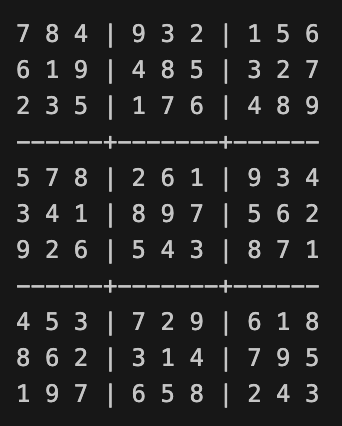
\includegraphics[width=0.3\textwidth]{"../Images/easy.png"}
    \caption{The CSP's solution to the easy sudoku puzzle.}
\end{figure*}

On the easy board, \textsc{Backtrack} was called 1 time and did not return \textit{failure} with \textsc{Minimum-Remaining-Values} (MRV) as the heuristic for \textsc{Select-Unassigned-Variable}. I tried with a simple "pick the first unassigned variable" heuristic as well. There was no difference in number of backtracs called, but that is because the easy board was solved by the first call to the \textsc{AC-3} algorithm. Thus the partila assignment passed to the first call of backtrack was complete and the assignment was returned. 

\subsection*{Medium}

\begin{figure*}[h!]
    \centering
    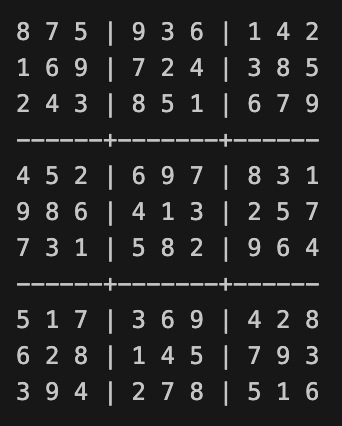
\includegraphics[width=0.3\textwidth]{"../Images/medium.png"}
    \caption{The CSP's solution to the medium sudoku puzzle.}
\end{figure*}

On the medium board, \textsc{Backtrack} was called 2 times and did not return \textit{failure} with MRV. With the systematic picker \textsc{Backtrack} was called 3 times, still with no \textit{failure} returns. Here the first call to \textsc{AC-3} solved most of the squares, but needed two more calls to solve the remaining unassigned squares. 

\newpage

\subsection*{Hard}

\begin{figure*}[h!]
    \centering
    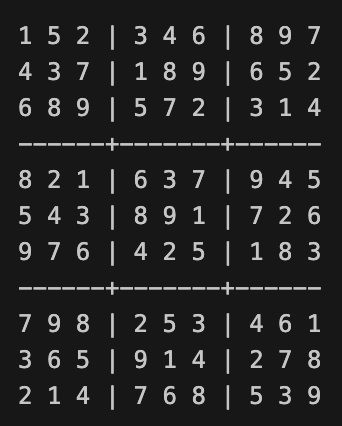
\includegraphics[width=0.3\textwidth]{"../Images/hard.png"}
    \caption{The CSP's solution to the hard sudoku puzzle.}
\end{figure*}

On the hard board, \textsc{Backtrack} was called 7 times and returned \textit{failure} 2 times. This is where the difference between MRV and the systematic picker became apparent. With the systematic picker, \textsc{Backtrack} was called 12 times and returned \textit{failure} 4 times. Almost twice as much as with MRV. This is probably due to MRV picking the variable that is most likely to cause a failure due to having the smalles domain of values of the unassigned variables. By doing this the search tree is pruned and the search becomes a smaller problem than before the pruning \cite{aima}. 

\subsection*{Very Hard}

\begin{figure*}[h!]
    \centering
    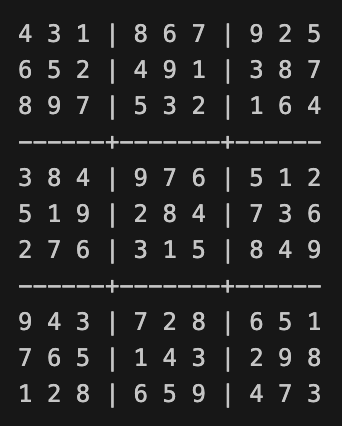
\includegraphics[width=0.3\textwidth]{"../Images/veryhard.png"}
    \caption{The CSP's solution to the vary hard sudoku puzzle.}
\end{figure*}

The very hard board had the same results as the hard board. With the MRV heuristic, \textsc{Backtrack} was called 7 times and returned \textit{failure} 2 times. With the systematic picker, as with the hard board, there were 12 calls to \textsc{Backtrack} and 4 returns of \textit{failure}. 

